\documentclass{beamer}
\usepackage[utf8]{inputenc}
\usepackage{graphicx}
\usepackage{natbib}
\usepackage{url}
\usetheme{Madrid}
\usecolortheme{beaver}
\bibliographystyle{apalike}

%\title[CTAP Demo]{Common Text Analysis Platform} 
%\subtitle{A Web-Based Tool Supporting Automatic Complexity Analysis}

\title{Comprehensive Complexity Analysis of Large-scale Learner Corpora with the Common Text Analysis Platform}

\author[X.B. Chen \& D. Meurers]{Xiaobin Chen, \\
	xiaobin.chen@uni-tuebingen.de \\
	\and 
	Detmar Meurers, \\
	dm@sfs.uni-tuebingen.de
}
\institute[T\"ubingen]{T\"ubingen University}
\date{\today}

\begin{document}
	 \frame{\titlepage}

	\begin{frame}
		\frametitle{Linguistic analysis of texts}

		(Automatic) Linguistic analysis has been widely used for: 
		\begin{itemize}
			\item assessing text readability 
			\item modeling processing difficulty of sentences
			\item analyzing/scoring student writings
			\item comparing language typologies and their historical development
			\item attributing authorship
			\item identifying native languages
			\item detecting plagiarism
			\item assessing answers to questions
			\item predicting diseases
			\item ...
		\end{itemize}
	\end{frame}


	\begin{frame}
		\frametitle{Existing tools for text analysis}

		A number of tools have been released in the past few years. e.g.

		\begin{itemize}
			\item Syntactic and Lexical Complexity Analyzers \citep{Lu-10}
			\item Cohmetrix \citep{McNamara.ea-14}
			\item Suite of Linguistic Analysis Tools
			\citep{Crossley.ea-16a,Crossley.ea-16b}, also
			\url{http://www.kristopherkyle.com/tools.html}
			\item Computerized Propositional Idea Density Rater
			\citep[CPIDR]{Brown.ea-08}. 
			\item ETS's TextEvaluator
			\url{https://texteval-pilot.ets.org/TextEvaluator/}
			\item Pearson's Reading Maturity Metric
			\item Text Analysis, Crawling, and interpretation Tool
			\citep[TACIT]{Dehghani.ea-16}
		\end{itemize}
	\end{frame}

	\begin{frame}
		\frametitle{Problems with existing tools}

		\begin{itemize}
			\item Limited usability of tools and analysis components
				  \begin{itemize}
					  \item OS-dependent standalone deployment
					  \item Source code release hard to use for non-programmers
					  \item Unfriendly user interface: command line interface,
							choice of features...
				  \end{itemize}
			\item Limited extensibility
				 \begin{itemize}
					 \item Close source commercial systems
					 \item Non-reusable analysis components
				 \end{itemize}
			\item Collaborative development difficult to implement
				 \begin{itemize}
					 \item Significant feature overlap
					 \item Duplication of efforts
				 \end{itemize}
			\item Feature proliferation, e.g.
				  \begin{itemize}
					  \item CohMetrix: 106 metrics
					  \item \citet{Vajjala-15}: $>$200 features for readability
					  assessment
				  \end{itemize}
		\end{itemize}
	\end{frame}

	\begin{frame}
		\frametitle{System demands}

		A system that is: 

		\begin{itemize}
			\item Web-based
			\item user-friendly, supporting real-life use by ordinary users
			\item comprehensive set of linguistic features
			\item freedom to choose extracted features
			\item modularized and reusable analysis components
		\end{itemize}
	\end{frame}

	\begin{frame}
		\frametitle{CTAP System Architecture}

		\centering
		\includegraphics[width=.8\textwidth]{img/ctap_architecture}
	\end{frame}

	\begin{frame}
		\frametitle{Corpus Manager}

		\begin{columns}
			\column{0.4\textwidth}
				 \centering
				  \includegraphics[height=.7\textheight]{img/corpus_manager}

			\column{0.6\textwidth}
				  Helps users manage the language materials that need to be
				  analyzed. 
				  \begin{itemize}
					  \item Folders: grouping corpora
					  \item Corpora: holding texts
					  \item Tags: labeling texts based on e.g. document genre,
					  target reader levels, etc.
				  \end{itemize}
		\end{columns}
	\end{frame}

	\begin{frame}
		\frametitle{Feature Selector}

		\begin{columns}
			\column{0.4\textwidth}
				  \includegraphics[height=.7\textheight]{img/feature_selector}

			\column{0.6\textwidth}
				The Feature Selector supports: 
				  \begin{itemize}
					  \item creating feature set to hold selected features
					  \item add/remove features from feature set
				  \end{itemize}

				  Developers are encouraged to participate in in feature
				  development at \url{https://github.com/ctapweb}.
		\end{columns}
	\end{frame}

	\begin{frame}
		\frametitle{Analysis Generator}

		\begin{columns}
			\column{0.4\textwidth}
				  \includegraphics[height=.7\textheight]{img/analysis_generator}

			\column{0.6\textwidth}
				 Each analysis extracts a set of features from the designated
				 corpus. 
				 The analysis generator is used to:
				  \begin{itemize}
					  \item create new analyses
					  \item run analyses and monitor their progress
					  \item export analysis results in CSV format
				  \end{itemize}
		\end{columns}
	\end{frame}


	\begin{frame}
		\frametitle{Result Visualizer}

				  \includegraphics[width=\textwidth]{img/result_visualizer}

					The Result Visualizer is a simple and intuitive module that
					plots analysis results for the user to visualize preliminary
					findings from the analysis.
	\end{frame}
	
	\begin{frame}
		\frametitle{Design features of CTAP}
		
		\begin{itemize}
			\item Consistent, easy-to-use, friendly user interface
			\item Modularized, reusable, and collaborative development of analysis
			components
			\item Flexible corpus and feature management
		\end{itemize}

	\end{frame}

	\begin{frame}
		\frametitle{System demo}

		\centering
		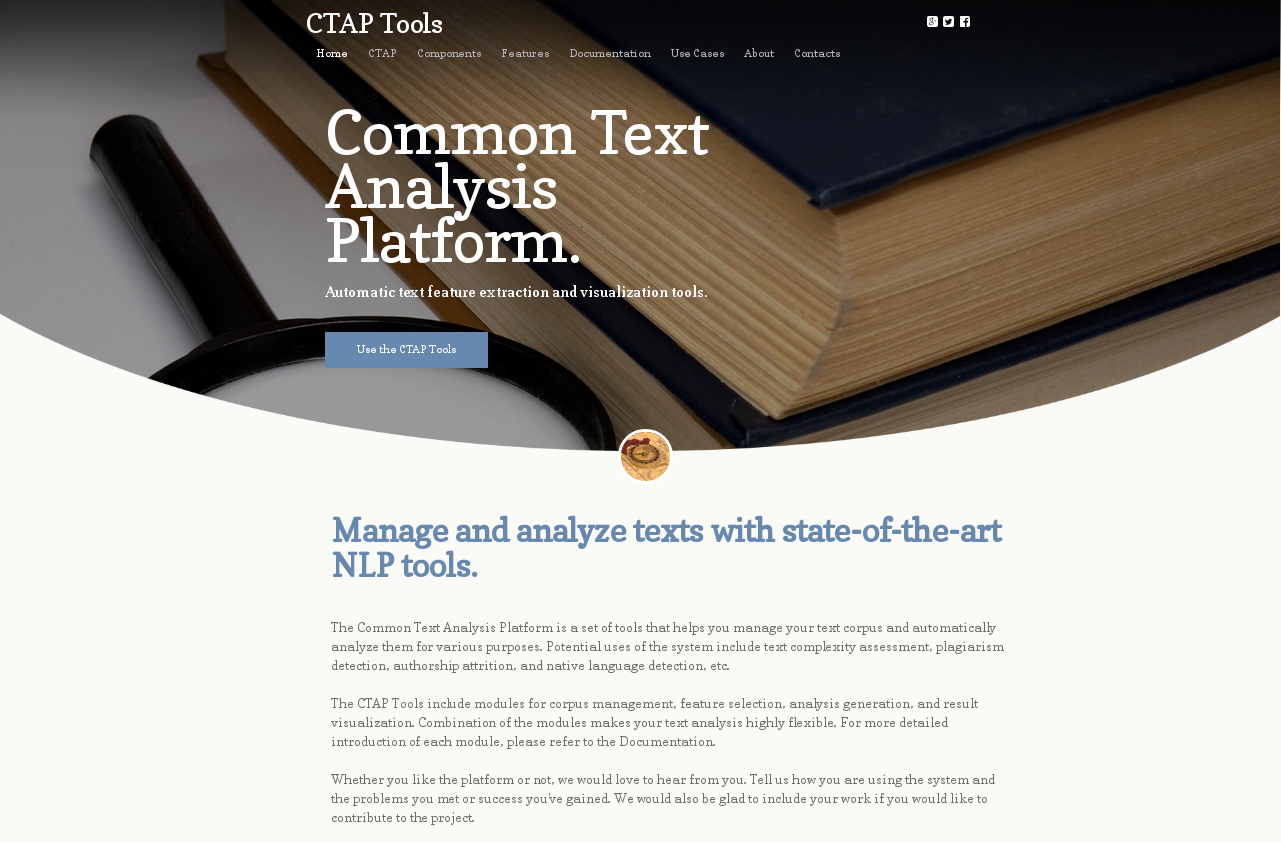
\includegraphics[width=.8\textwidth]{img/ctapweb}

		\url{http://ctapweb.com}
	\end{frame}

	\begin{frame}
		\frametitle{Outlook}

		\begin{itemize}
			\item Populating the system with more features
			\item Replicating studies that involved text analysis to validate the
			system and identify other function needs 
			\item Model construction functionality (machine learning)
			\item Acurracy measures
			\item API supporting analysis of multiple languages (en, de, es,
				 fr...), non-plain text file formats, etc. 
		\end{itemize}

		More details available in the paper:

		\scriptsize{
			 Chen, X. B., \& Meurers, D. (2016). CTAP: A Web-based tool supporting
			 automatic complexity analysis. In D. Brunato, F. Dell'Orletta, G.
			 Venturi, T. François, \& P. Blache (Eds.), \textit{Proceedings of the
			 Computational Linguistics for Linguistic Complexity Workshop at the
			 26th International Conference on Computational Linguistics (COLING
		2016)}, Osaka, Japan, 11 December (pp. 113-119). The International
		Committee on Computational Linguisitcs.
		}

	\end{frame}

	\begin{frame}
		\frametitle{References}
		\tiny
		\bibliography{bibliography}

	\end{frame}
	
\end{document}

